
\printMiniToc


\normalInfo{Level design}{Le \anglicisme{level design} est l'art de créer des niveaux bien équilibrés, fun à jouer et variés. C'est l'art de bien disposer les obstacles, récompenses et bâtiments pour que la difficulté soit adaptée. La carte doit présenter suffisamment de challenge pour motiver les joueurs, sans être excessivement difficile ce qui les empêcherait d'avoir une bonne expérience du jeu.}

\warningInfo{Niveaux déjà préparés}{Seuls les premiers niveaux du jeu sont définis de manière détaillée. Le reste du jeu n'est qu'hypothétiquement décrit à la fin de ce chapitre.}

\section{Premier acte}
\label{sec:premierActe}

\subsection{Redel, le quartier pauvre}
Le premier niveau se déroule dans le quartier pauvre, nommé Redel (voir les cartes \ref{fig:murtosLaGrande} et \ref{fig:carteQuartierPauvre}). Il se situe à l'extrême sud de \nomVille. C'est le quartier le plus sale, où vivent les gens les plus pauvres.

Le coin sud-est du quartier est occupé par une énorme usine gouvernementale. L'accès à cette dernière est formellement interdit et des gardes surveillent en continu son entrée. De plus, elle crache sur le quartier des fumées toxiques, particulièrement malsaines à respirer.

\subsubsection{Un \enquote{bastion vert}}
Les dernières personnes à croire en la Nature habitent les maisons les plus isolées, au sud de Redel. Ces gens cachent cependant leur croyance, de peur d'être persécutés. N'ayant plus vu une plante depuis des années, ils commencent à oublier ou à sombrer dans la superstition.

Un des trois sanctuaires de la Nature, celui de Tia, est caché dans ce quartier. Pour y accéder, un passage secret existe dans la maison située juste au nord de ce jardin caché. Cette dernière est habitée par Maïnin, un vieil homme sage qui a gardé l'esprit clair et lucide.

\subsection[Niveau 1 -- Course-poursuite avec la garde]{Premier niveau -- Course-poursuite avec la garde}
\label{sec:coursepoursuiteGarde}
\warningInfo{Un niveau d'importance}{Le premier niveau est crucial, c'est à la fois la scène d'exposition, l'opportunité de découvrir l'univers du jeu et l'apprentissage nécessaire des contrôles. S'il est bien réussi, fluide, le joueur pourra prendre plaisir à jouer et s'attacher à son personnage.}

Dans le premier niveau d'\nomJeu, le joueur incarne Kida, l'héroïne, et est accompagnée de Lenaï, sa grande s\oe ur. Les tous premiers instants servent à l'apprentissage des commandes: se déplacer, courir, s'accroupir, sauter, etc.

Puis viens l'élément déclencheur: deux gardes qui passent par l'avenue marchande, oublient négligemment un petit coffre au bord de l'étalage où ils viennent d'acheter de quoi manger. Kida ne peut s'empêcher de voler le coffre. Mais au moment de commettre son délit, les gardes reviennent, ayant noté leur inadvertance. À la vue des deux s\oe urs, ils leur hurlent d'arrêter et la course-poursuite s'engage immédiatement.

Le joueur doit passer à temps les obstacles qui lui sont présentés afin de pouvoir s'enfuir. Le niveau ne doit présenter qu'une faible difficulté pour permettre au joueur à la fois de s'habituer aux commandes et d'avoir une première impression aussi bonne que possible.

À la fin du niveau, Kida s'enfuit avec le coffre mais Lenaï est capturée. Cet élément sera la cause des multiples péripéties qui s'ensuivront dans cette histoire.

\normalInfo{Niveau de type \anglicisme{alley}}{Ce niveau est dit de type \anglicisme{alley}. À savoir, le joueur n'est pas libre de se balader selon sa bonne volonté. À l'inverse, pour réussir le niveau, il doit suivre avec succès un chemin prédéfini.}

\subsection[Niveau 2 -- À la recherche de Lenaï]{Deuxième niveau -- À la recherche de Lenaï}
\label{sec:rechercheLenai}
\warningInfo{Objets à débloquer dans ce niveau}{\begin{itemize}
		\item Bâton de bois
		\item Trois sorts majeurs
		\item Tyrolienne
		\item Sarbacane
		\item Une recette de poison
	\end{itemize}
}

Le deuxième niveau débute le jour suivant. Kida part à la recherche de sa s\oe ur. Cette quête va cependant être entravée par le fait que la garde a bouclé les sorties du quartier pour retrouver le coffre volé; tout le monde est fouillé. Ainsi, l'héroïne est bloquée dans Redel. Faute de mieux, elle cherche à ouvrir le coffre volé, qui semble avoir nettement plus de valeur que ce qui aurait pu être supposé dans un premier temps.

La première tâche du joueur sera d'ouvrir le coffre. Pour cela, il faudra trouver du métal, s'introduire dans la boutique du serrurier absent par les toits et utiliser ses machines pour créer une clé adaptée. Lorsque le coffre s'ouvre, un étrange animal en bondi. C'est la première rencontre avec un esprit de la Nature: Tia, l'écureuil vif et sauvage. La créature dit à Kida d'aller voir Maïnin, le vieux sage, puis s'enfuit en courant.

Le vieil homme, qui est en fait le gardien de l'accès au sanctuaire, y introduit la jeune fille (il faut résoudre un puzzle pour activer le passage). Kida rencontre Tia, qui lui explique les bases du fonctionnement de l'énergie verte, lui confie les trois premiers totems et le bâton de bois (voir les sections sur le \nameref{chap:gameplay}). Elle lui parle également d'un passage secret au c\oe ur du quartier naturel. Il donne accès à la rivière, puis à la tour de Gaamon dans laquelle Lenaï est sûrement enfermée.

Pour accéder à ce quartier, il faut résoudre toute une série de quêtes et de sous-quêtes pour finalement débloquer le passage indiqué par un \enquote{?} sur la maison mitoyenne de celle du cordonnier.

Les Naturels confieront à Kida la sarbacane, quelques dards et sa première recette de poison. Si le joueur a déjà collectionné suffisamment d'ingrédients, il peut confectionner des dards supplémentaires. Ils ouvrent ensuite le passage situé sous la statue de Gaamon, au milieu de la place. L'héroïne peut ainsi accéder à la rivière.

\normalInfo{Niveau de type \anglicisme{island}}{Ce niveau, à l'inverse du précédent, représente un niveau de type \anglicisme{island}. Cela signifie que le joueur est libre de ses mouvements et peut aller où bon lui semble. Un autre terme pour décrire ce type de niveau serait semi open-world\definition.}


\begin{figure}[ph!]
	\centering	
	\subfloat[Plan du quartier pauvre]{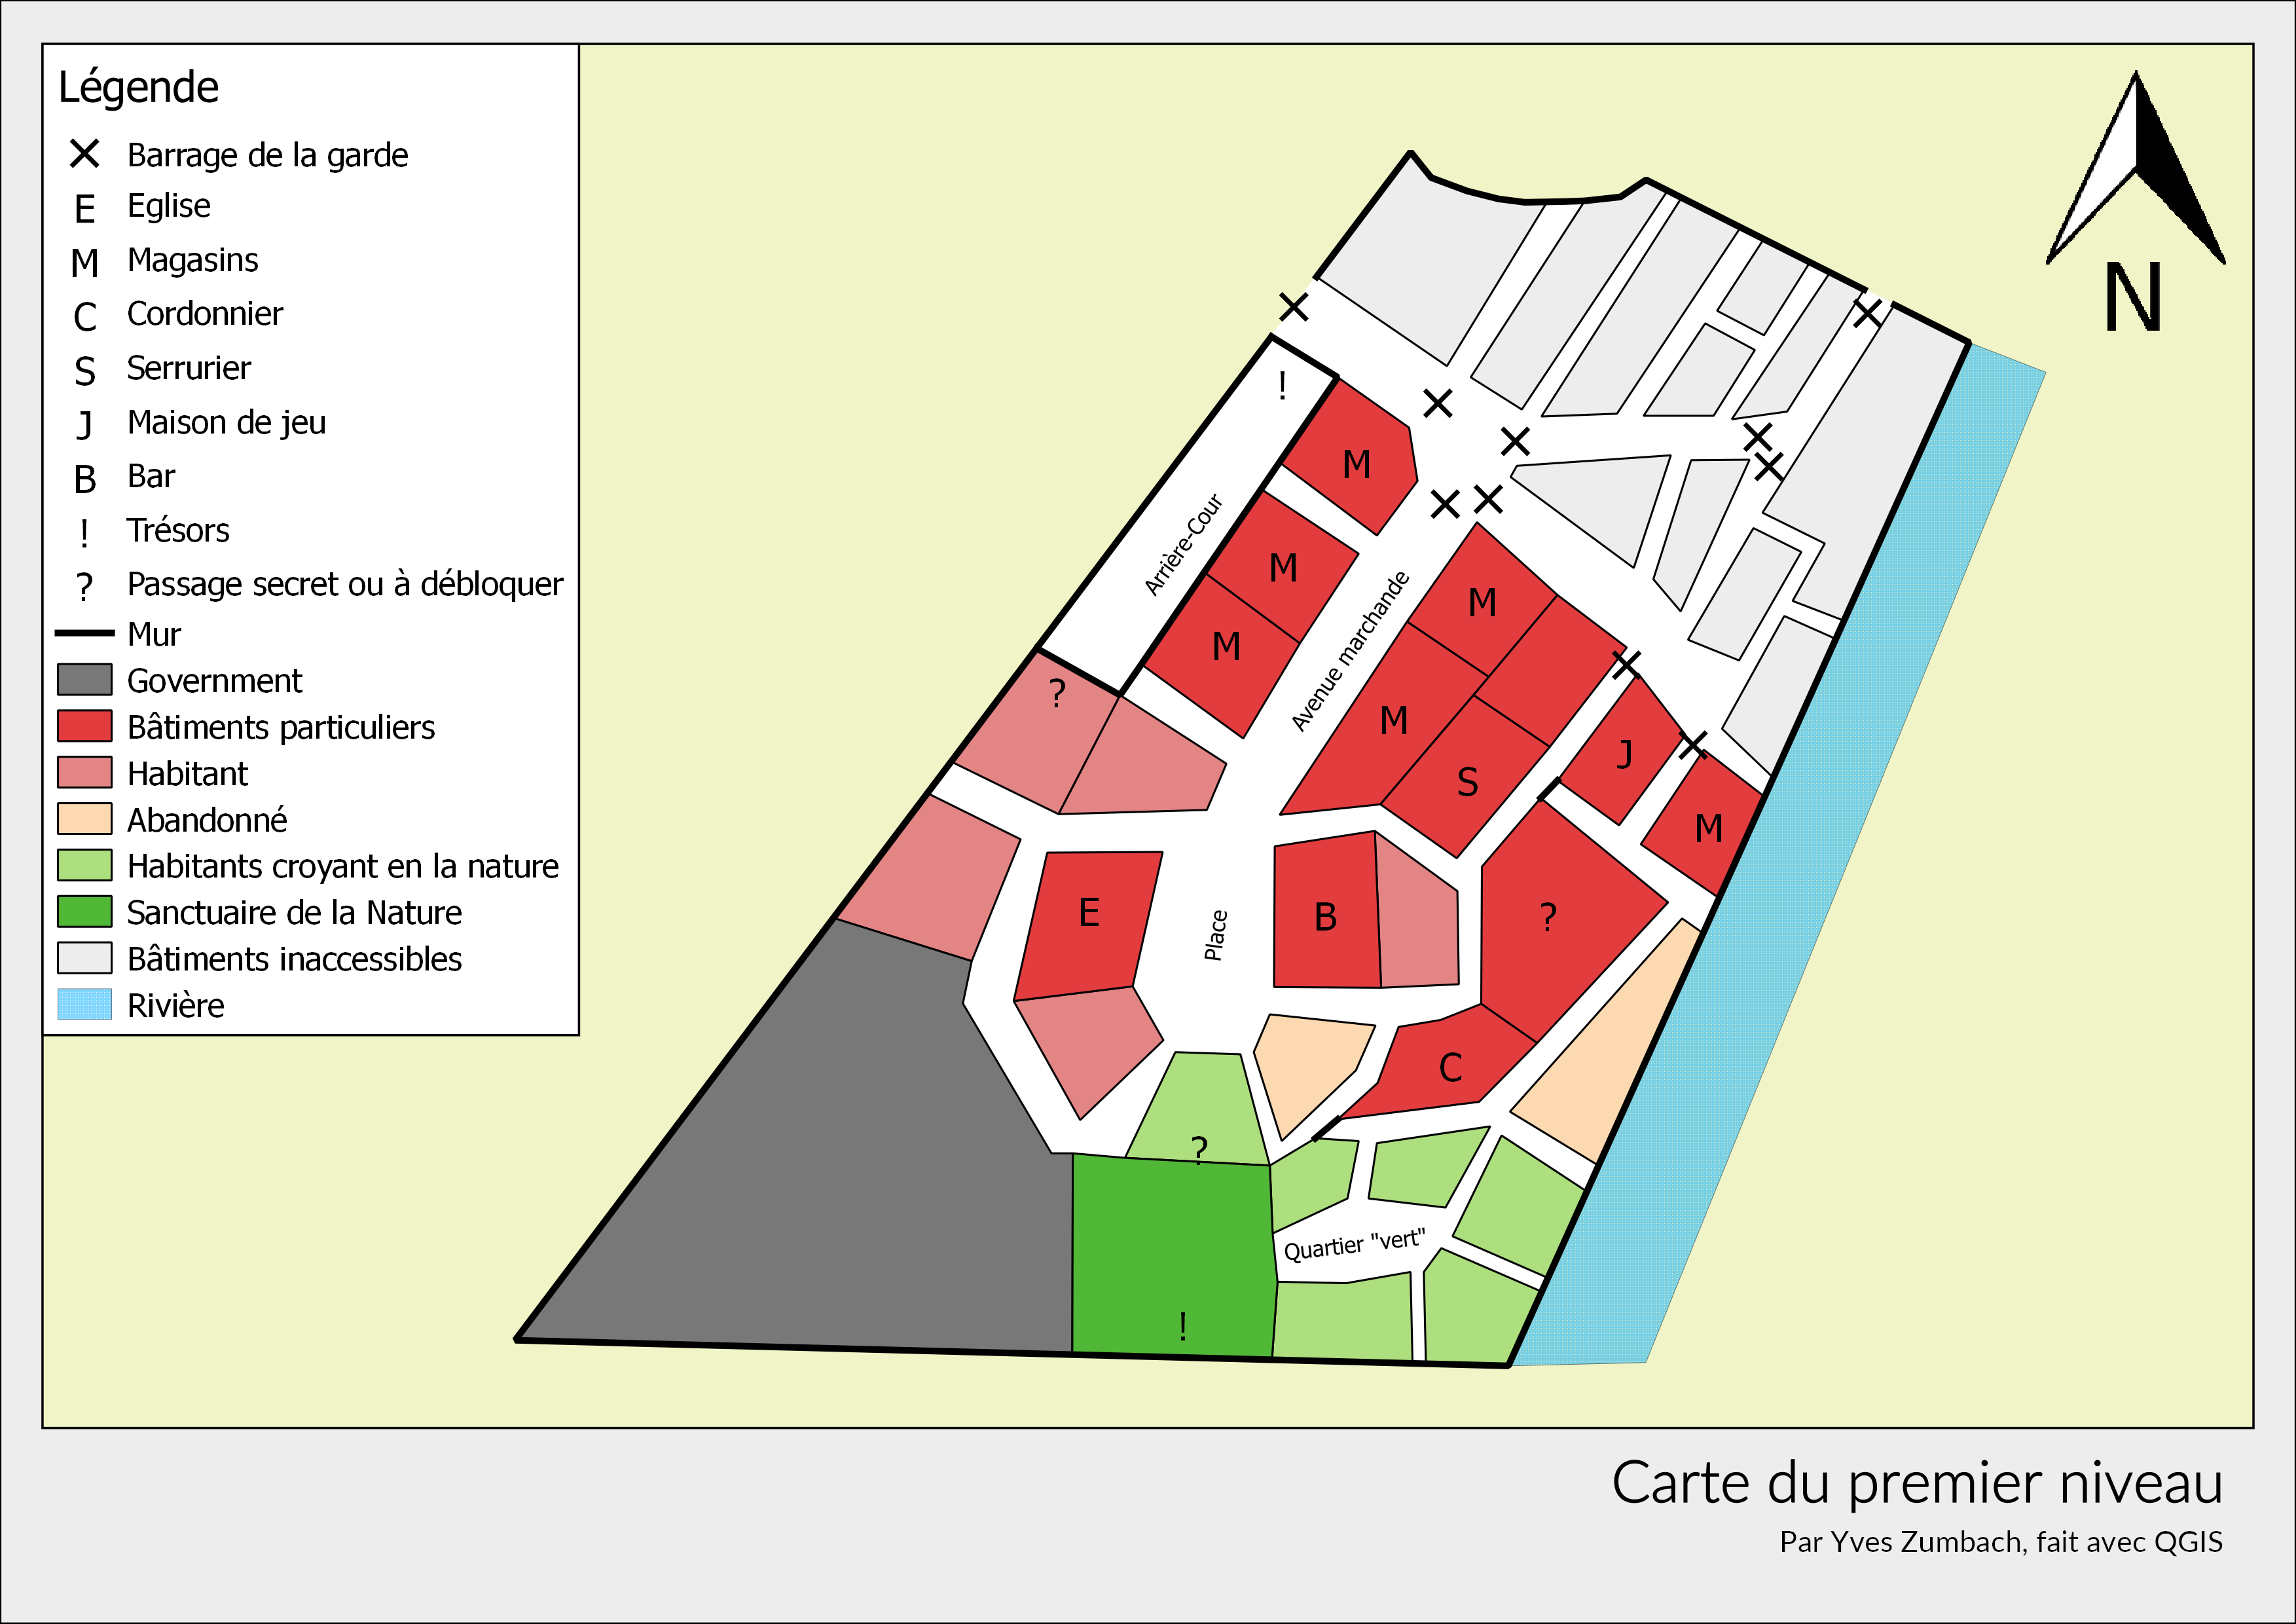
\includegraphics[width=\textwidth]{images/LevelDesign/cartePremierNiveauIndicationsGameplay.png}}
	
	\subfloat[Plan des toits]{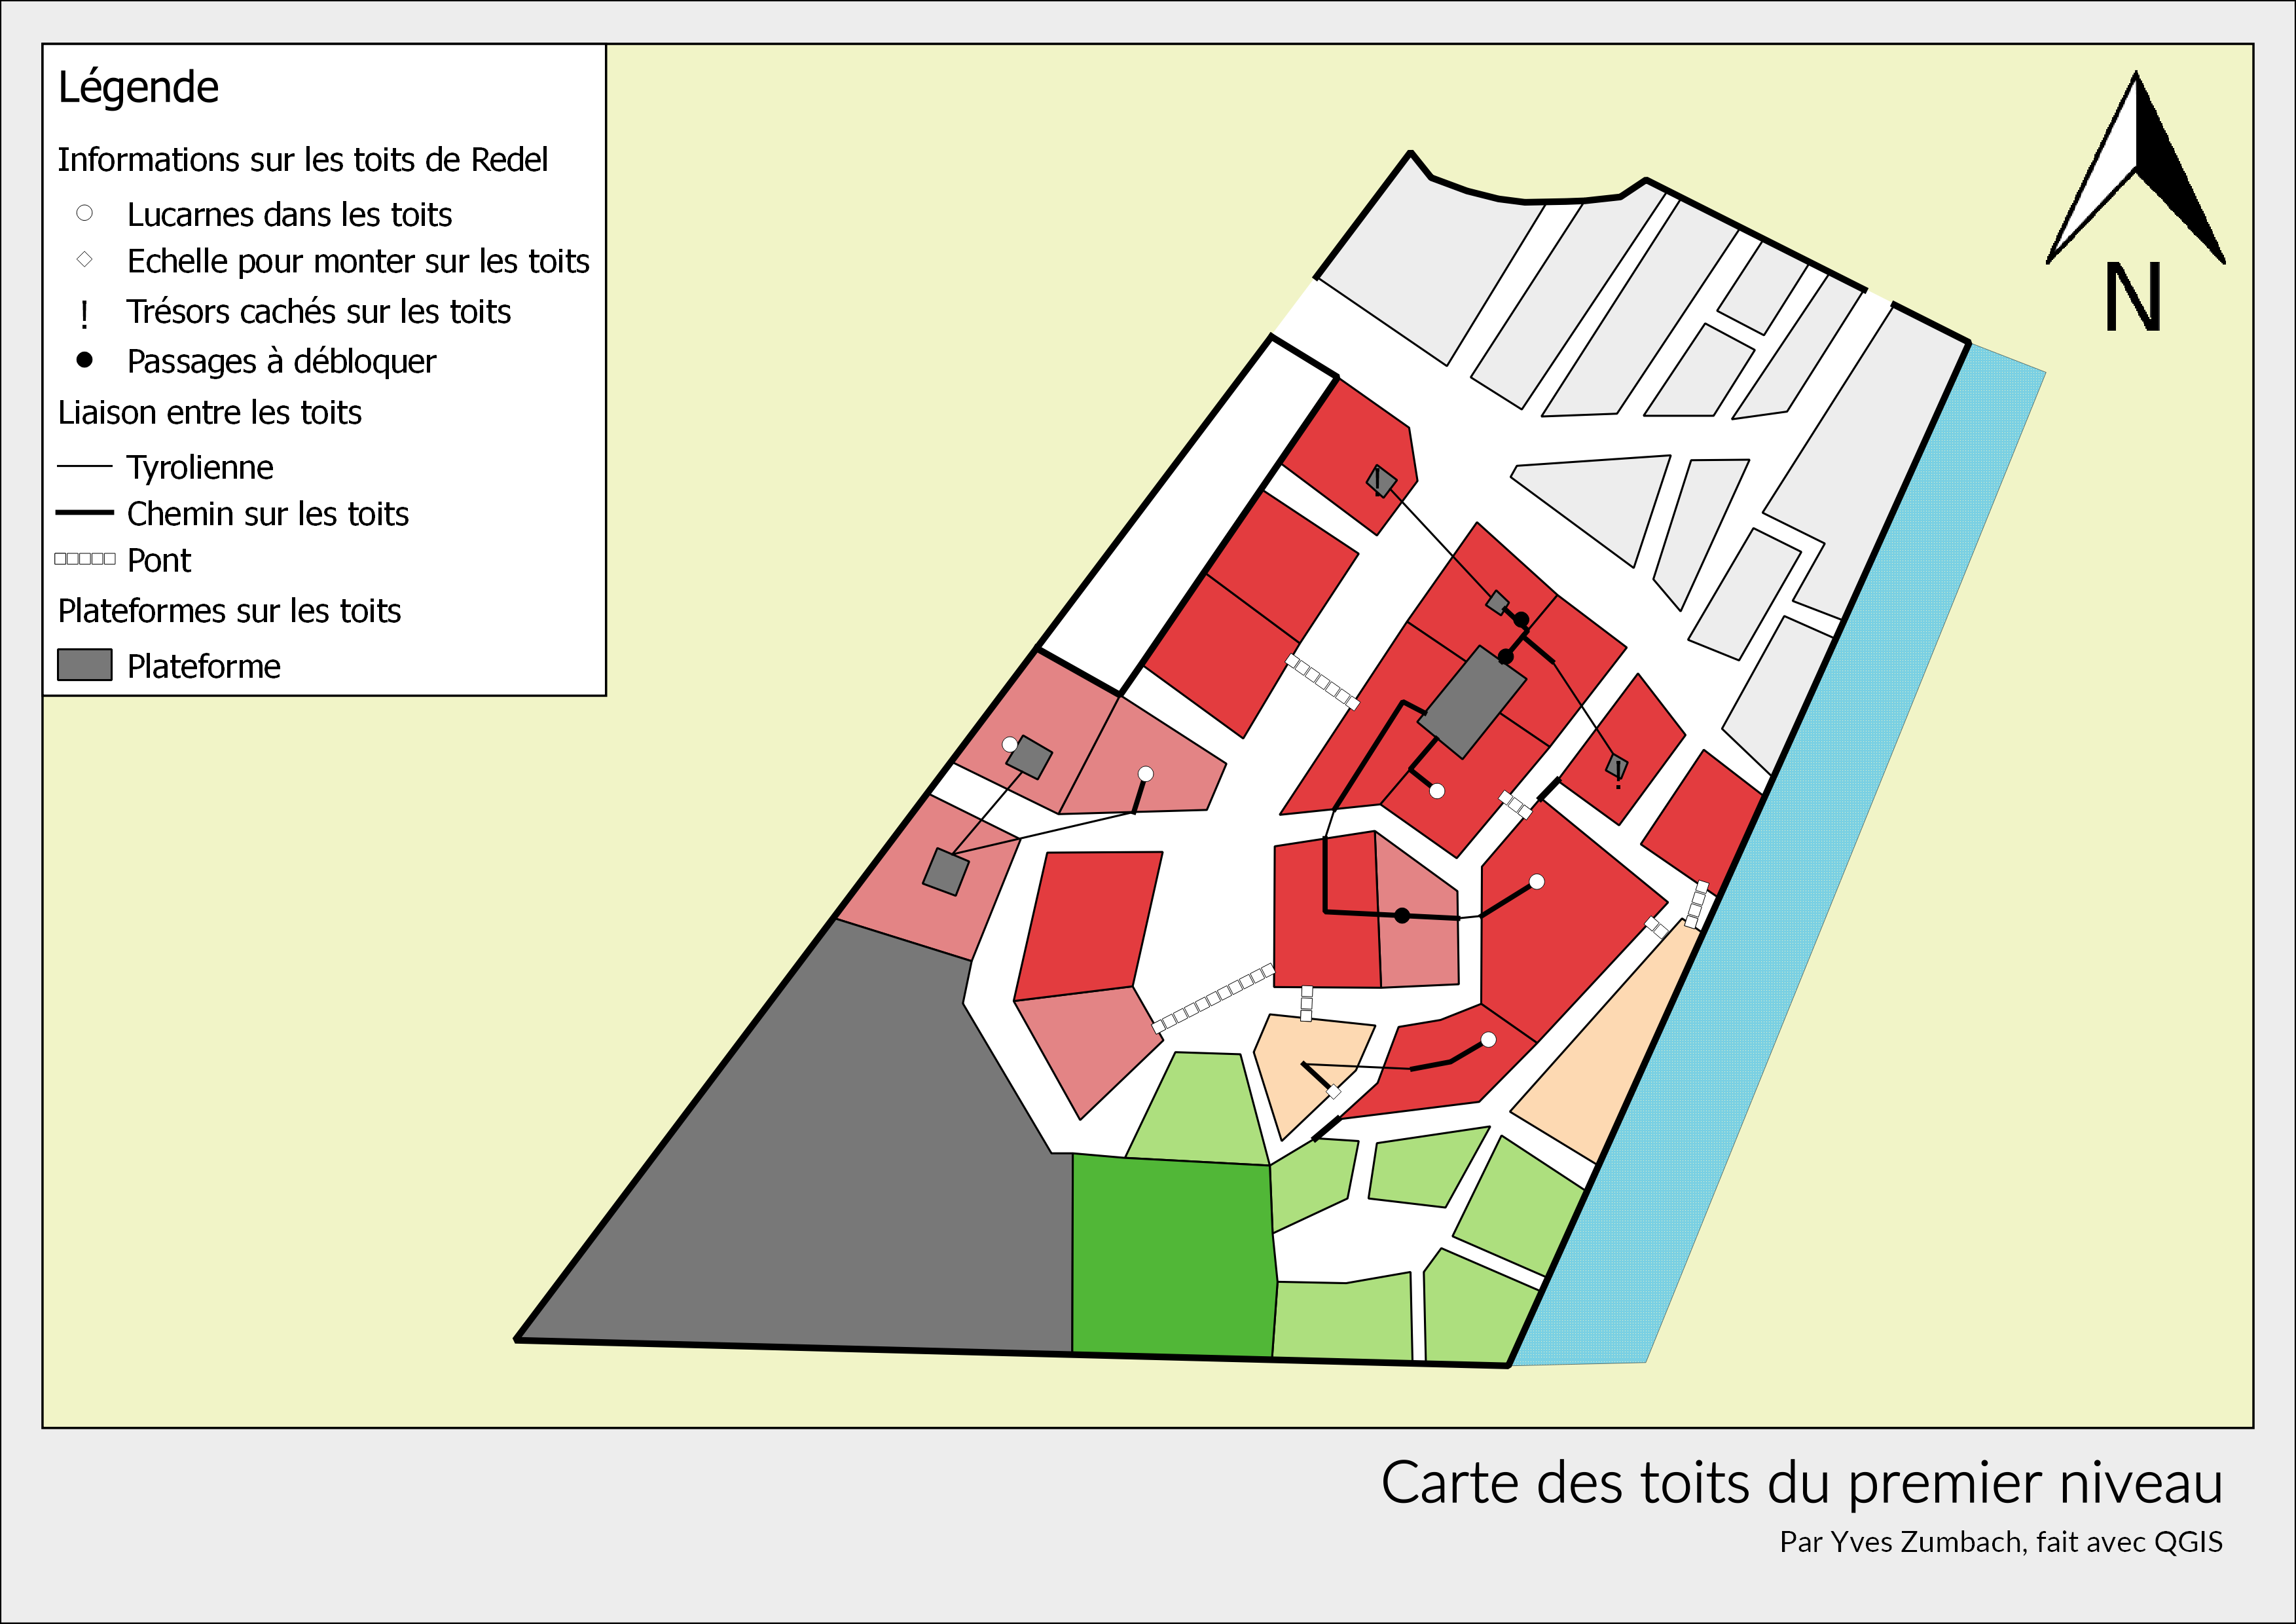
\includegraphics[width=\textwidth]{images/LevelDesign/carteToitsPremierNiveau.png}}
	
	\caption{\label{fig:carteQuartierPauvre}Cartes du premier niveau}
\end{figure}


\subsection[Niveau 3 -- Dans l'antre du démon]{Troisième niveau -- Dans l'antre du démon}
\label{sec:entreDemon}
Kida pénètre dans le château de Gaamon par les souterrains. Ce niveau est un temple\definition. Il s'agira donc de trouver les cachots où Lenaï pourrait être enfermée. Cela en résolvant des puzzles\definition\ pour accéder aux pièces suivantes et éviter les ennemis (se référer à la partie \enquote{\nameref{chap:gameplay}} pour plus de détails).

Les objectifs intermédiaires du niveau seront de trouver la carte, collecter des objets et des clés afin de pouvoir ouvrir les portes vers les salles suivantes.

Finalement, en arrivant aux cachots, Kida ne trouvera que des cellules vides... Aucune trace de Lenaï. C'est à ce moment que le boss\definition\ apparaît sous la forme d'une grande femme en armure. Le combat s'engage immédiatement. Si Kida se défend du mieux qu'elle peut, elle ne peut résister face à son adversaire parfaitement équipée pour le combat, aux armes aiguisées et techniques évoluées. Elle finit par se faire renverser et atterrit durement sur le sol, désarmée. L'antagoniste lève son arme afin de porter le coup de grâce. Mais l'espace d'un instant, un éclair de doute traverse les yeux de la guerrière. Instantanément, Kida reconnait sa grande s\oe ur\ sous le masque terrifiant qu'elle porte: c'est contre Lenaï qu'elle se bat! L'ainée ne peut se résoudre à assassiner sa petite s\oe ur. Kida profite de l'ouverture pour s'enfuir à toute vitesse, se précipite vers la fenêtre la plus proche et saute droit dans les douves... à l'extérieur de la ville.

\criticalInfoDarkRed{Importance du troisième niveau}{Le troisième niveau est véritablement la clé de voute de cette histoire. On y découvre que Lenaï est passée du côté de Gaamon. Cet élément capital sera le point de départ de l'histoire d'\nomJeu.}

\section{Deuxième acte}
\label{sec:deuxiemeActe}
Kida se retrouve hors des murs pour la première fois de sa vie. Elle va devoir s'habituer à un nouveau mode de vie plus rural, plus sauvage et découvrir les populations environnant \nomVille. Ces personnes sont pour la plupart des renégats ou des paysans ayant fui lors de la création de la ville. La vie est très dure. Elle apprendra ici la légende fantastique du peuple des \nomNaturels s. Pour sauver sa s\oe ur, elle se mettra à leur recherche et finira par découvrir, caché au fond d'une forêt, un très ancien temple à l'architecture étrange, gracieuse mais sortie tout droit d'un autre âge: un temple \nomNaturels. C'est en haut de ce dernier qu'elle découvrira un engin volant aussi vieux que le temple. Il la conduira sur les hauts-plateaux, où le peuple persécuté a trouvé refuge.

\section{La suite}
Une fois arrivée chez les Telurans, Kida découvre que le peuple magnifique en lequel elle espérait n'est plus que l'ombre de lui-même. Les persécutions incessantes de Gaamon ont fini d'achever les dernières merveilles de ce peuple: le palais royal tombe en ruine, les secrets de l'énergie verte, cette science magnifique, se perdent chaque jour, un par un. 

{\color{red} A terminer!!!!!} 

\subsection{Jouer Lenaï}
La plupart des niveaux sont joués avec Kida. Cependant, certains utiliseront Lenaï comme personnage; ce qui apporte de multiples avantages: réutilisation des contenus, points de vue diversifiés, aperçu de la vie de Lenaï. Ce dernier point est celui qui a le plus de valeur pour moi. Il permet d'approfondir le gameplay: lorsqu'on joue Lenaï, on est forcé d'exécuter les ordres de Gaamon, il faut donc compléter les missions données par le grand ennemi du jeu. Le tyran commande à ses soldats des missions à l'éthique hautement critiquable: collecter des impôts énormes chez les habitants, aller éradiquer la Nature sur une surface toujours grandissante autour de la cité, etc. Ces missions seront l'occasion de proposer un choix au joueur quant à leur résolution. Par exemple pour la collecte des impôts, le joueur pourra retourner les maisons des habitants incapables de payer pour trouver jusqu'à la dernière pièce, une solution simple et efficace, ou alors faire l'effort de  trouver lui-même des pièces pour aider les personnes les plus en difficulté. Ces niveaux seront aussi l'occasion d'explorer la relation entre Lenaï et Gaamon, à la fois paternelle et ambivalente car Lenaï, bien qu'elle soit \enquote{ensorcelée}, perçoit bien que ce qu'elle fait n'est pas correct.

\subsection{Des batailles aériennes}
Les véhicules, et plus particulièrement les dirigeables, sont un élément important du Steampunk. Il pourrait être intéressant de créer des batailles aériennes entre des aéronefs telurans datant de leur époque glorieuse, propulsé à 'énergie verte et des forteresses volantes humaines.



